\documentclass[]{article}
\usepackage{lmodern}
\usepackage{amssymb,amsmath}
\usepackage{ifxetex,ifluatex}
\usepackage{fixltx2e} % provides \textsubscript
\ifnum 0\ifxetex 1\fi\ifluatex 1\fi=0 % if pdftex
  \usepackage[T1]{fontenc}
  \usepackage[utf8]{inputenc}
\else % if luatex or xelatex
  \ifxetex
    \usepackage{mathspec}
    \usepackage{xltxtra,xunicode}
  \else
    \usepackage{fontspec}
  \fi
  \defaultfontfeatures{Mapping=tex-text,Scale=MatchLowercase}
  \newcommand{\euro}{€}
\fi
% use upquote if available, for straight quotes in verbatim environments
\IfFileExists{upquote.sty}{\usepackage{upquote}}{}
% use microtype if available
\IfFileExists{microtype.sty}{%
\usepackage{microtype}
\UseMicrotypeSet[protrusion]{basicmath} % disable protrusion for tt fonts
}{}
\usepackage[margin=1in]{geometry}
\ifxetex
  \usepackage[setpagesize=false, % page size defined by xetex
              unicode=false, % unicode breaks when used with xetex
              xetex]{hyperref}
\else
  \usepackage[unicode=true]{hyperref}
\fi
\hypersetup{breaklinks=true,
            bookmarks=true,
            pdfauthor={Erik Bulow},
            pdftitle={Arbetslogg 2016 vecka 10},
            colorlinks=true,
            citecolor=blue,
            urlcolor=blue,
            linkcolor=magenta,
            pdfborder={0 0 0}}
\urlstyle{same}  % don't use monospace font for urls
\usepackage{color}
\usepackage{fancyvrb}
\newcommand{\VerbBar}{|}
\newcommand{\VERB}{\Verb[commandchars=\\\{\}]}
\DefineVerbatimEnvironment{Highlighting}{Verbatim}{commandchars=\\\{\}}
% Add ',fontsize=\small' for more characters per line
\usepackage{framed}
\definecolor{shadecolor}{RGB}{248,248,248}
\newenvironment{Shaded}{\begin{snugshade}}{\end{snugshade}}
\newcommand{\KeywordTok}[1]{\textcolor[rgb]{0.13,0.29,0.53}{\textbf{{#1}}}}
\newcommand{\DataTypeTok}[1]{\textcolor[rgb]{0.13,0.29,0.53}{{#1}}}
\newcommand{\DecValTok}[1]{\textcolor[rgb]{0.00,0.00,0.81}{{#1}}}
\newcommand{\BaseNTok}[1]{\textcolor[rgb]{0.00,0.00,0.81}{{#1}}}
\newcommand{\FloatTok}[1]{\textcolor[rgb]{0.00,0.00,0.81}{{#1}}}
\newcommand{\ConstantTok}[1]{\textcolor[rgb]{0.00,0.00,0.00}{{#1}}}
\newcommand{\CharTok}[1]{\textcolor[rgb]{0.31,0.60,0.02}{{#1}}}
\newcommand{\SpecialCharTok}[1]{\textcolor[rgb]{0.00,0.00,0.00}{{#1}}}
\newcommand{\StringTok}[1]{\textcolor[rgb]{0.31,0.60,0.02}{{#1}}}
\newcommand{\VerbatimStringTok}[1]{\textcolor[rgb]{0.31,0.60,0.02}{{#1}}}
\newcommand{\SpecialStringTok}[1]{\textcolor[rgb]{0.31,0.60,0.02}{{#1}}}
\newcommand{\ImportTok}[1]{{#1}}
\newcommand{\CommentTok}[1]{\textcolor[rgb]{0.56,0.35,0.01}{\textit{{#1}}}}
\newcommand{\DocumentationTok}[1]{\textcolor[rgb]{0.56,0.35,0.01}{\textbf{\textit{{#1}}}}}
\newcommand{\AnnotationTok}[1]{\textcolor[rgb]{0.56,0.35,0.01}{\textbf{\textit{{#1}}}}}
\newcommand{\CommentVarTok}[1]{\textcolor[rgb]{0.56,0.35,0.01}{\textbf{\textit{{#1}}}}}
\newcommand{\OtherTok}[1]{\textcolor[rgb]{0.56,0.35,0.01}{{#1}}}
\newcommand{\FunctionTok}[1]{\textcolor[rgb]{0.00,0.00,0.00}{{#1}}}
\newcommand{\VariableTok}[1]{\textcolor[rgb]{0.00,0.00,0.00}{{#1}}}
\newcommand{\ControlFlowTok}[1]{\textcolor[rgb]{0.13,0.29,0.53}{\textbf{{#1}}}}
\newcommand{\OperatorTok}[1]{\textcolor[rgb]{0.81,0.36,0.00}{\textbf{{#1}}}}
\newcommand{\BuiltInTok}[1]{{#1}}
\newcommand{\ExtensionTok}[1]{{#1}}
\newcommand{\PreprocessorTok}[1]{\textcolor[rgb]{0.56,0.35,0.01}{\textit{{#1}}}}
\newcommand{\AttributeTok}[1]{\textcolor[rgb]{0.77,0.63,0.00}{{#1}}}
\newcommand{\RegionMarkerTok}[1]{{#1}}
\newcommand{\InformationTok}[1]{\textcolor[rgb]{0.56,0.35,0.01}{\textbf{\textit{{#1}}}}}
\newcommand{\WarningTok}[1]{\textcolor[rgb]{0.56,0.35,0.01}{\textbf{\textit{{#1}}}}}
\newcommand{\AlertTok}[1]{\textcolor[rgb]{0.94,0.16,0.16}{{#1}}}
\newcommand{\ErrorTok}[1]{\textcolor[rgb]{0.64,0.00,0.00}{\textbf{{#1}}}}
\newcommand{\NormalTok}[1]{{#1}}
\usepackage{graphicx,grffile}
\makeatletter
\def\maxwidth{\ifdim\Gin@nat@width>\linewidth\linewidth\else\Gin@nat@width\fi}
\def\maxheight{\ifdim\Gin@nat@height>\textheight\textheight\else\Gin@nat@height\fi}
\makeatother
% Scale images if necessary, so that they will not overflow the page
% margins by default, and it is still possible to overwrite the defaults
% using explicit options in \includegraphics[width, height, ...]{}
\setkeys{Gin}{width=\maxwidth,height=\maxheight,keepaspectratio}
\setlength{\parindent}{0pt}
\setlength{\parskip}{6pt plus 2pt minus 1pt}
\setlength{\emergencystretch}{3em}  % prevent overfull lines
\providecommand{\tightlist}{%
  \setlength{\itemsep}{0pt}\setlength{\parskip}{0pt}}
\setcounter{secnumdepth}{5}

%%% Use protect on footnotes to avoid problems with footnotes in titles
\let\rmarkdownfootnote\footnote%
\def\footnote{\protect\rmarkdownfootnote}

%%% Change title format to be more compact
\usepackage{titling}

% Create subtitle command for use in maketitle
\newcommand{\subtitle}[1]{
  \posttitle{
    \begin{center}\large#1\end{center}
    }
}

\setlength{\droptitle}{-2em}
  \title{Arbetslogg 2016 vecka 10}
  \pretitle{\vspace{\droptitle}\centering\huge}
  \posttitle{\par}
  \author{Erik Bulow}
  \preauthor{\centering\large\emph}
  \postauthor{\par}
  \predate{\centering\large\emph}
  \postdate{\par}
  \date{07 mars 2016}


% Redefines (sub)paragraphs to behave more like sections
\ifx\paragraph\undefined\else
\let\oldparagraph\paragraph
\renewcommand{\paragraph}[1]{\oldparagraph{#1}\mbox{}}
\fi
\ifx\subparagraph\undefined\else
\let\oldsubparagraph\subparagraph
\renewcommand{\subparagraph}[1]{\oldsubparagraph{#1}\mbox{}}
\fi

\begin{document}
\maketitle

{
\hypersetup{linkcolor=black}
\setcounter{tocdepth}{2}
\tableofcontents
}
\section{Förberedelser}\label{forberedelser}

\begin{Shaded}
\begin{Highlighting}[]
\CommentTok{# Try it out!}
\KeywordTok{memory.limit}\NormalTok{(}\DecValTok{50000}\NormalTok{)}
\end{Highlighting}
\end{Shaded}

\begin{verbatim}
## [1] 50000
\end{verbatim}

\begin{Shaded}
\begin{Highlighting}[]
\KeywordTok{options}\NormalTok{(}\DataTypeTok{samplemetric.log =} \OtherTok{TRUE}\NormalTok{)}
\KeywordTok{set.seed}\NormalTok{(}\DecValTok{123}\NormalTok{)}
\end{Highlighting}
\end{Shaded}

\section{2016-03-07}\label{section}

\subsection{Läsning av (Cattin 1980)}\label{lasning-av-cattin1980}

Handlar bl a om multiple correlation coefficient i CV. Står att
skattningar för regressionen sker via OLS. Gör skillnad på fixed och
random model men skriver om båda.

Är långt ifrån enda källan men också här ges den ganska pedagogiska
formeln för \(R^2\) som vi kanske kan återanvända:

\[R^2 = 1 - \frac{\sum_{i = 1}^N (Y_i + \hat{Y}_i)^2}{\sum_{i = 1}^N (Y_i + \bar{Y}_i)^2}\].

Nämner att man tidigare funnit att adjusted \(R^2\) enl (Wherry 1931)
(dvs (Ezekei 1929)) har en bias som mest uppgår till \$.1 / N \$ om
\(x\) fixed (men tar inte hänmsyn till \(\rho\) \ldots{} kanske därmed
en referens att kolla upp?)

Nämner också att (Olkin and Pratt 1958) är biased ty oändlig serir
trunkeras.

Nämner att det även finns flera källor som utvecklat adjusted-versioner
spec för cross-validatiln men att även dessa tenderar vara biased. Här
rekommenderas olika versioner för fixed resp randmo regression.

Gör också egna simuleringar i fallet då \(p = 1\), dvs för vanliga
\(r^2\). Finner att bias är ganska liten men att korrigernig kan behövas
då \(\rho \leq .4, N < 50\).

Förespråkar att \(R^2\) justeras mha ngn föreslagen formell hellre än
via CV då detta anges ge mindre bias (och förstås mindre
beräkningsintensivt).

Poängterar vikten av att OLS används vid skattning och menar att terorin
falerar vid t ex stepwise linear regression och liknande (ty
prediktorerna måste väljas på förhand).

\subsection{Läsning av (Crocker 1972)}\label{lasning-av-crocker1972}

Behandlar multiple correlation coefficient (dock \(r\) och inte
\(R^2\)). Poängterar att (enl (Wishart, Kondo, and Elderton 1931))
\[E[R^2|\rho = 0] = \frac{p}{n-1}\]

Detta betyder att \(E[R^2]\) kan hamna nära 1 för stora \(p\) och små
\(n\). Detta kanske kan vara viktigt då det samtidigt är pedagogiskt.

Nänmer att ref {[}3{]} ger konfidensintevall för \(\rho\) för olika
\(p, n\) och att detta även utvecklats i ref {[}6{]}.

Noterar att \(R^2|\rho = 0 \sim F = \frac{R^2/p}{(1-R^2)/(n-p-1)}\).

\subsection{Läsning av (R. A. Fisher 1928)}\label{lasning-av-fisher1928}

Tycks vara ngt slags original för sample-fördelning av multilpe
correlation coefficient.

Ficher skriver att han blev tvungen att betrakta helt nya fördelningar.
Dessa var dessutom olika för olika parametervärden men efter hand insågs
att det fanns ett mönster som förenade dem.

Påpekar att om
\(Y = \beta_0 + \sum_{i = 1}^p \beta_i x_i + \varepsilon\) så kommer
\(cor(Y, \hat{Y}) = \xi(\mathbf{x})\) för godtycklig linjärkombination
\(\xi\). Därmed reduceras problemet att finna den multipla
korrelationskoefficienten till att hitta korrelationskoefficienten
mellan två variabler.

Artikeln är extremt formelrik men en viktig slutsats är att den multipla
korrelationen ej beror på hela korrelationsmatrisen mellan alla
variabler utan bara på den multilpa korrelationen i populationen
varifrån sampling sker.

Dock är själva fördelningsformeln oerhört krånglig och utvecklas olika
för olika parametervärden. Känns inte smo att detta kan ha ngn smo helst
praktisk nytta i dess här föreslagna form. Nyttjar bla också
Bessel-funktioner. Kollade också bland de artiklar som refererar till
denna men hittade ingen som tycks ha utvecklat metoden (även om det
fnins gott om referenser).

\subsection{Läsning av (Wishart, Kondo, and Elderton
1931)}\label{lasning-av-wishart1931}

Handlar om multiple correlation coefficient med samples från N.
Behandlar väntevärde och varians av sådana \(R^2\).

\[\bar{R}^2 = 1 - \frac{b}{a + b}F(1, 1, a+b+1, \rho^2)\] och för
\(\rho\) ges då \[\bar{R}^2 = \frac{a}{a + b}\] och för \(\rho = 1\)
\[\bar{R}^2 = 1\]

där \(a = p/2\) (dvs hälften av antalet kovariater) och
\(b = (n - p - 1)/2\) (avrundat till heltal).

Påtalas också att (R. a Fisher 1924) gav den ungefärliga
approximationen:

\[E[R^2] = \bar{R}^2 = a - \frac{b}{a + b}(1-\rho^2)\] och att detta är
en ganska bra approximation åtm då n stort.

Vi kan väl här konstatera att den bias som här presenteras tycks ara den
bias för vilken (Ezekei 1929) justerar!? Dock hänvisade E själv till
tidigare opublicerade källor så kan inte se exakt att det var just
därför.

F.ö. har vi väl sedan tidigare liknande resultat för det icke mulipla
fallet och nu får vi ngt som liknar detta.

\textbf{OBS!!!} Detta känns väl som ett ganska intressant och viktigt
resultat att ta med sig!?

Vi får också enl (19):

\[\sigma^2_{R^2} = \frac{b(b+1)(1-\rho^2)^2}{(a+b)(a + b +1)}F(2,2,a+b+2,\rho^2) - \frac{b^2(1-\rho^2)^2}{(a+b)^2}F^2(1,1,a+b+1, \rho^2)\]

I och med dessa uttryck skulle vi alltså kunna kolla att den bias vi får
överrensstämmer med detta! :-)

Nänmer också att det finns en approximation på detta uttryck sedan
tidigare men visar att den inrte är tillräcklig utan att detta exakta
uttryck krävs, åtminstone för små stickprov.

Sedan beräknas även motsvarande för \(R\) och till artikeln finns ett
editorial appendix med tabellverk över olika \(n\) och \(p\).

Enligt appendix ges formlerna istället direkt map \(n, p\) enl (i) och
(ii). Nänmer att olika förf använder olika beteckningar. T ex Fisher
\(n_1, n_2\), Wishart \(a, b\) appendixet \(N, n\) och vi \(n, p\) och
att dessa behöver transformeras en aning mellan de olika skrivsätten.

På det hela taget en viktig artikel känns det som.

\subsection{Läsning av (Kramer 1963)}\label{lasning-av-kramer1963}

Låt \(X_{ij} (i = 1, 2, \ldots, k; j = 1, 2, \ldots, n)\) beteckna ett
sample av \(n\) observationer dragna slumpmässigt från icke-singulär
\(k\)-variat normalfördelning. Då är

\[r_{hm} = \frac{n\sum_{j = 1}^n X_{hj}X_{mj}-(\sum_{j = 1}^nX_{hj}) \sum_{j = 1}^nX_{mj}}{
\sqrt{
   \big[
       n 
       \sum_{j = 1}^n
       X_{hj}^2-
       (\sum_{j = 1}^n)^2
    \big]
    \big[
      n
      \sum_{j = 1}^n X_{mj}^2 - 
      (\sum_{j=1}^n X_{mj})^2
    \big] 
  }
}\]

den vanliga korrelationskoefficienten mellan kovariaterna \(X_h\) och
\(X_m\). Låt sedan \(P\) vara determinanten av korrelationsmatrisen av
de enkla korrelationerna och \(P'\) dess första kofaktor. Då ges den
multipla korrelationskoefficienten mellan \(X_i\) och
\((X_2, \ldots, X_k)\) som den ickenegativa kvadratroten:

\[R = \sqrt{1 - \frac{P}{P'}}\]

Därefetr ges delvis en formel för konfidensnitervall (uttrycks dock inte
helt explicit) samt tabelluppgifter för denna beronde på
stickprovsstorlek och antal kovariater.

\subsection{Läsning av (Montgomery and Morrison
1973)}\label{lasning-av-montgomery1973}

Skriver explicit att storleken av bias för unadjusted \(R^2\) kan vara
tillräckligt stor för att orsaka rejäla tolkningsproblem.

Ger en approximation av \(E[R^2|n, k, \rho^2]\) och beräknar biasen för
olika givna \(n, k, \rho\). Observera att detta gjordes då det kanske
fortfranade var lite svårare att använda den exakta formeln, vilket ju
enligt ovan egentligen är att föredra. Vi skulle ju kunna komplettera
dessa beräkningar med värden från den exakta formeln.

Biasen blir allra värst då \(\rho = 0\).

Väldigt bra och pedagogisk artikel. Saknar dock illustrerande grafer,
vilket vi skulle kunna tillföra.

Nämner att för adjusted \(R^2\) gäller (approximativt):
\[bias(\bar{R}^2) = - \frac{\rho^2(1-\rho^2)(1-2\rho^2)}{n}\] dvs bias
\textgreater{} 0 om \(\rho \geq 1/2\) och \textless{} 0 om
\(\rho \leq 1/2\). Denna bias är dock väldigt liten, den beror inte på
\(p\) och blir som mest \(.1/n\). Största bias uppstår då
\(\rho = .2, .8\). Bias = 0 då \(\rho = 0, 1/2, 1\).

Poängterar att det inte räcker med stort n för att undvika bias utan att
det krävs att förhållandet mellan p och n är bra.

\subsection{Läsning av (Ozer 1985)}\label{lasning-av-ozer1985}

Förklarar och kritiserar tolkning av \(r^2\) mha Venn-diagram (refererar
till folk som gjort det tidigare). I denna tolkning (som också uttrycks
algebraiskt) mäts korrelation som delmängder av element som förekommer i
bvåde X och Y (dvs diskreta fall).

Känns lite off-topic men kanske kan vara värt att nänma som en
alternativ förklaringsmodell etc. Läser inte färdigt.

\subsection{Fundernigar kring hur själva rtikeln kan
skrivas}\label{fundernigar-kring-hur-sjalva-rtikeln-kan-skrivas}

Det går att modifiera template för Word-dokument som genereras av Knitr:
\url{https://vimeo.com/89562453}

Det finns även en del färdiga \LaTeX-mallar i paketet \texttt{rticles}
som kan väljas via
\texttt{File\ \textgreater{}\ New\ file\ \textgreater{}\ R\ Markdown...}.
Man kan även skapa egna templates enligt:
\url{http://rmarkdown.rstudio.com/developer_document_templates.html}

Har vi tur så kanske den tidsskrift vi vill submitta till erbjuder
template i ngt lättanvänt format. Elsviewer-artiklar har t ex en mall i
\texttt{rticles}-paketet.

\section{2016-03-08}\label{section-1}

\subsection{Läsning am betafördelning på
Wikipedia}\label{lasning-am-betafordelning-pa-wikipedia}

\url{https://en.wikipedia.org/wiki/Beta_distribution}

OBS! Berör den vanliga, centrerade. Mode (antimode få
\(\alpha, \beta < 1\)) kan beräknas men median saknar closed form. Finns
olika förenklade formler för median givna i artikeln.

Medelvärde ges av: \[\mu = E[X] = \frac{1}{1 + \frac{\beta}{\alpha}}\]

Om \(\alpha = \beta \Rightarrow \mu = 1/2\).

Det bör alltså ganska intressant att underseröka för vilka värden
betafördelningen slår över från U-shaped till den ``vanliga formen''.
Tror också att detta har nämnts ngnstans i litteraturen men kan tyvärr
inte minnas var.

Variansen ges av:
\[var(X) = E[(X-\mu)^2] = \frac{\alpha \beta}{(\alpha + \beta)^2(\alpha + \beta + 1)}\]

Man kan också parametrisera fördelningen mha
\(\mu, \nu = \alpha + \beta (\nu > 0)\):
\[\alpha = \mu \nu, \beta = (1 - \mu)\nu\]

Betafördelningen utvecklades av Pearson men kallades då
Pearson-fördelning typ 1 och hade 4 parametrar. Dock går det att
transformera denna fördelning till vanlig beta (på ngt sätt).

Betafördelningen tycks ha nämnts första gången 1911.

Parametrarna \(\alpha, \beta\) kan lättast skattas mha momentmetoden
(det var f.ö. en skism mellan Pearson och Fisher just angående huruvida
man skulle använda detta eler maximum likelihood, vilket dock tycks mer
komplicerat).

\[\hat{\alpha} = \bar{x}\big( \frac{\bar{x}(1-\bar{x})}{\bar{v}-1}\big), \beta = (1-\bar{x})\hat{\alpha}, \textrm{ if } \bar{v} < \bar{x}(1-\bar{x})\]

\subsection{Googlande}\label{googlande}

Finns en relevant fråga på SO som kan knytas till formel för
ickecentralitetsparametern i ickecentrala betafördelningen:
\url{http://stats.stackexchange.com/questions/58107/conditional-expectation-of-r-squared/58133\#58133}

Bygger dock på ganska avancerad matematik som jag har lite svår att ta
till mig. Refererar också till: (Walck 2007) vars avsn 30 behandlar
ickecentral betafördelning men in te ger ngn bra formel för \(\lambda\).
Hjälp för tolkning av SO-posten:
\url{http://www.math.uah.edu/stat/expect/Matrices.html} Med hjälp av
dessa formler borde vi kunna få en formel för fördelningen av \(R^2\).
Dock görs inte detta i själva frågan utan här gör man istället en
approximation för ett upper bound av \(E[R^2]\). Är osäkler på varför.
Man får ju en analytisk formel för ickecentral beta och denna i sin tur
har en closed form för dess mean!?

Dock kan också noteras att \(\lambda\) beror på väntevärdet av X. Att vi
ovan sett att betafördelningen ger en bra approximation till
fördelningen kan nog rimligtivs bero på att vi har väntevärde = 0 för
den data vi simulerat. Resultatet kan nog därmed förväntas bli
annorlunda med andra väntevärden. Kanske ngt att udersöka iofs men
kanske ett stickspår.

\textbf{OBS!!!} Noterar nu att \(\lambda\) ju faktiskt beror på \(X\),
dvs på stickprovet. Detta innebär ju att vi i praktiken är tillbaka i
vår sedan tidigare kända situation. Dock har vi här ett beroende på hela
\(X\), dvs en designmatris som vi kanske kan ta från vårt ursprungliga
stora sample. Således har vi kanske trots allt inte ett beroende på den
ensklda stickprovet!?

Det som sägs är:

\begin{quote}
Consider the simple linear model:
\end{quote}

\[\pmb{y}=X'\pmb{\beta}+\epsilon\]

\begin{quote}
where \(\epsilon_i\sim\mathrm{i.i.d.}\;\mathcal{N}(0,\sigma^2)\) and
\(X\in\mathbb{R}^{n\times p}\), \(p\geq2\) and \(X\) contains a column
of constants.
\end{quote}

\begin{quote}
\(R^2\sim\mathrm{B}(p-1,n-p,\lambda)\) where
\(\mathrm{B}(p-1,n-p,\lambda)\) is a non-central Beta distribution with
non-centrality parameter \(\lambda\) with
\end{quote}

\[\lambda=\frac{||X'\beta-\mathrm{E}(X)'\beta1_n||^2}{\sigma^2}\]

Dock misstänker jag här att \(X'\) kan vara sammanblandat med \(X\) och
att det således borde vara \(X \beta\) istf \(X' \beta\). Har vi inte
\(\beta\) borde vi istället kunna skatta \(X\beta\) med hattmatrisen,
dvs \(X(X'X)^{-1}X'Y\) \ldots{} eller är det lika bra att börja om från
början med data som helt följer modellen?

OBS! Denna (eller åtm liknande formel finns ockspå som (12) i (Helland
1987). Är väl därmed bättre att utgå från den som faktiskt publicerad
referens.

OBS!!! \(X\) härrör fortfarande till just aktuellt sample ty \(\lambda\)
växer med \(n\) :-(

Dock kan vi anta att centralitetsparametern = 0 då \(E[X] = 0\) och då
approximera med vanlig betafördelning. (Men gäller nog inte föfr lite
mer komplicerade fördelningar, gissar att det inte räcker att bara
standardisera resp parameter \ldots{} eller?)

\subsection{Läsning av (Helland 1987)}\label{lasning-av-helland1987}

Om tolkning av \(R^2\) i regression. Argumenterar för att \(R^2\) bara
kan tolkas korrekt just då kovariaterna är random (då detta är bästa
sättet att få en heltäckande bild av X). Skriver att det finns en del
statistiker som avråder från att i huvud taget titta på \(R^2\).
Föreslår approximativt konfidensintervall för populationskoefficienten
för korrelation. Observerar att adjusted \(R^2\) faller inom intervallet
men inte den vanliga. Utgår från modeller med intercept och
ickekorrelerade fel. Bygger på matrisformler.

Ger också \(\rho^2\) på formen:
\[\rho^2 = \frac{\sum_{i = i}^p \beta_ix_i}{var(y)}\]

Härleder också ickecentralitetsparametern
\[\lambda = \frac{\beta'X'_0X_0\beta}{\sigma^2}\] Detta sägs ge en
konditional distribution av \(R^2\) givet \(X_0\) för random \(X\). För
en unconditional fördelning krävs dock fördelningsantagande för \(X\).
Detta beräknades redan av(R. A. Fisher 1928) men är för krångligt för
att kunna användas. En approximation har dock givits av en Gurland 1968
(ej läst):
\[k = \frac{\rho^2}{1-\rho^2}, a = \frac{(n-k)k(k+2) + p}{(n-1)k +p}, v = \frac{(n-1)k+p}{a}\Rightarrow \frac{R^2}{1-R^2} \approx \frac{(n-1)k +p}{n-p-1}F_{v, n-p-1}\]
Denna approximation har sedan visat sig fungera bra. Utifrån denna
approximation konstrueras sedan konfidensintervall. Den formel som då
föreslås beror dock på \(\rho\). Numeriska metoder används och
konvergens uppnås ofta efter 3-4 itterationer. Resultatet härav blir
väldigt bra överrensstämmande med tidigare teoretiskt uträknade
motsvarande värden. Artikelns beskrivning av metoden är antagligen
tillräcklig för att själv kunna återimplementera den men det känns ändå
lite krångligt.

\subsection{Läsning av (Rodgers and Nicewander
1988)}\label{lasning-av-rodgers1988}

Innehåller en del historia. Artikeln skrevs för att fira att det var ca
100 år sedan regression infördes. Återkommer till de kändisar vi sett
sedan tidigare men i organiserad form. Redan 1920 skrev f.ö. Pearson
``Note on the history of correlation''.

Skriver också att konceptet både är ett av de mest använda men också
mest missbrukade inom statistik.

Artikeln presenterar sedan 13 olika tolkningar av \(r\) men bara under
vissa förenklade förutsättningar, såsom endast bivariat fördelning:

\begin{enumerate}
\def\labelenumi{\arabic{enumi}.}
\tightlist
\item
  den anliga algebraiska formeln
\item
  som standardiserad kovarians
\item
  som lutningen (slope) i regressionsmodell
\item
  geomertiskt medelvärde
\item
  roten av proportion of variability accounted for
\item
  mean cross product of standardized variables
\item
  vinkeln mellan två standardiseerade regressionslinjer
\item
  funktion av vinkeln mellan de två variabelvektorerna
\item
  \ldots{}
\end{enumerate}

En del av de övriga känns lite väl teoretiska \ldots{}

\section{2016-03-09}\label{section-2}

Jobbar hemifrån med att läsa lite artiklar.

\subsection{Läsning av (Wasserstein and Lazar
2016)}\label{lasning-av-wasserstein2016}

Artikeln handlar om att ASA till viss del sätter ner foten och tar
avstånd för överdrivet bruk av p-värden. Kan var värt att bara nämna att
det inte är helt självklart att syftet med att undersöka fördelningen
för R2 är att kunna skapa hypoteser etc.

\subsection{Läsning av (Nambury S Raju et al.
1997)}\label{lasning-av-raju1997}

Om multiple regression. Om CV och OLS. Vill jämföra korrigeringar av
\(\rho\) baserat på:

\begin{itemize}
\tightlist
\item
  CV
\item
  Formula-based (dvs adjusted).
\end{itemize}

Påtalar att även om en skattning \(r\) för \(\rho\) är unbiased
(antingen via CV eller formell), betyder det inte per automatik att
också skattningen \(r^2\) av \(\rho^2\) är unbiased.

Antar X fixed men \(\varepsilon \sim N\).

Påtalar att om syftet är prediction bör \(\rho_c\) skattas mha CV. I så
fall gäller dock att \(\rho_c^2 < \rho^2\). Skillnaden beror på skillnad
mellan CV-sample och population. Här är \(\rho_c^2\) också ett
teoretiskt värde och även här nämns att \(R^2\) överskattar detta.
Nämner att (Wherry 1931) först nämna att shrinkage innebär att också
\(R_c^2<R^2\).

Nämner att Huberty 1994, Snijders 1996 och Yung 1996 undersökt metoder
för signifikanstest av \(R^2\) och att detta vid denna tidpunkt var ngt
ganska nytt. Kanske värt att kolla upp?

Har i andra artiklar argumenterats för att adjustmentmetoder för fixed X
är tillämpliga också för random X om \(n > 50\).

Här står att adjusted enl (Ezekei 1929) utvecklades av (Wherry 1931) och
att dessa formler således skiljer sig lite. Ger en historik och
sammanfattning av de olika adjusted-skattningarna som presenterats och
undersökyts.

refererar til studie som visat att CV sämre än formula based.
Jämförelser med 4 och 8 kovariater och stickprovsstorlekar
\textgreater{}= 50. Men även då vissa svårigheter (rekommenderar
\textgreater{}= 250). Detta underbyggs också med referenser till fler
liknande studier. Dock poängteras att CV kan vara bättre just för
predektion.

De simuleringar so mgjort dittills tycks i de flesta fall begränsas till
populationsstorlekar om 5000.

En del simuleringar har också gjorts på väldigt små stickprov och med
varierande \(\rho\).

Konstateras att bootstrap och jack-knife kan rekommenderas först för n
\textgreater{}= 100.

Skriver också mkt om EW jmfrt med OLS, vilket jag inte läser då det
ligger utanför nuvarande intresse.

Slutsats att formula based rekommenderas. Kan dock inte rekommendera ngn
enskild då det trots alla jämförelser inte funnits ngn jämförelse som
täckt samtliga.

\textbf{Slutsats:} Denna artikel är väldigt omfattande gällande referat
av tidigare studier för jämförelser av olika adjustments!

\subsection{Läsning av (Nakagawa and Niki
1992)}\label{lasning-av-nakagawa1992}

Behandlar endast \(r\) men gör det för icke-normalfördelad population.
Nämner att det utvecklats metoder/algoritmer för beräkning av flertalet
moment för fördelning av r men att högre moment kräver väldigt mkt
algebra. Utgår från cumulants
(\url{https://en.wikipedia.org/wiki/Cumulant}) (dvs \(\ln(M)\)) där M =
moment istf moments men gör koplpingar tillbaka till moments. Denna
artikel utvecklar nu approximationer till de fyra första momenten mha
Edgeworth-expansions
(\url{https://en.wikipedia.org/wiki/Edgeworth_series}), vilket är en
metod att approximera sannolikhetsfördelningar mha just cumulants.
Använder också delta-metoden

\subsection{Fixar Mendeley}\label{fixar-mendeley}

Känner att det uppståt ett visst behov av att försöka få lite mer
ordning i Mendeley så lägger rätt mkt tid på detta. Lyckas bl a fixa ett
automatsynkat bibtex-bibliotek som jag hoppas kunna knyta direkt till
loggen etc. Har också slagit samman dubletter, rensat bort ickerelevanta
artiklar och gått igenom så att all information stämmer. Ett ganska
stort jobb faktiskt men hoppas att det kan vara värt det.

\subsection{Läsning av (N S Raju et al.
1999)}\label{lasning-av-raju1999}

Kan ses som en uppföljning till (Nambury S Raju et al. 1997) men med
egen simuleringsstudie. KOmmer fram till att adjusted (Ezekei 1929) är
bästa sättet att justera.

Utgår från verkligt dataset med nästan 85000 fall. Fördel framför
datorsimulerat data att det kan avspegla verkigheten bättre i form av
att inte helt följa teoretiska modeller etc.

Sample sizes 25, 40, 60, 80, 100, 150, and 200 för 501 samples.

Motiverar små stickprovsstorlekar:

\begin{quote}
Based on 125 reported validity studies, Callender, Osburn, Greener, \&
Ashworth (1982) found that 33\% of the studies reported mean Ns below 50
and that 51\% of the studies reported mean Ns between 50 and 100.
\end{quote}

Jämförde 16 different formulas (seven formulas originally developed
\(\rho^2\) for estimating population multiple correlation and nine
formulas initially developed for estimating population cross-validity).
Jämförde:

\begin{quote}
mean of bias (MB) and mean of squared bias (MSB). Note that MSB reflects
both MB and the SD of bias. The means and SDs of bias and squared bias
were obtained separately for each combination of estimation procedure,
N, and population parameter that was estimated.
\end{quote}

Table 2 faktiskt väldigt intressant. Visar tydligt jämförelser mellan
olika värden och där tydligt att (Ezekei 1929) väldigt bra. Table 3
visar ännu tydligare mean bias och att (Ezekei 1929) är bäst samt att
formula bättre än CV. Motsvarande resultat ges för mean squared bias.
Detta visas även grafiskt.

Jag läser inte de delar av artikeln som berör skattningar mha CV eller
EW utan hoppar direkt till diskussion.

Refererar till att även tidigare jämförelser visat att (Ezekei 1929)
bäst och detta både för vanlig regression och stepwise.

Studien erkänner dock att en brist är att man inte använt olika \(\rho\)
eller olika \(p\) då detta ju varit fixt för ett faktiskt dataset.
Likaså då data kommer från ickenormal-fördelning etc. Begränsar sig
också till least square (ej ridge regression, PCA etc) men det gäller ju
för oss också.

Här kan vi ju också påminna oss själva om att (Skidmore and Thompson
2011) just undersökte fler \(\rho\) och olika sorters fördelningar. De
fann att (Olkin and Pratt 1958) var bäst men att (Ezekei 1929) var
ungefär lika bra. Slutsatsen blir väl då trots allt att rekommendera
(Ezekei 1929), dels då den är enklare, dels då den beskrivs både på
Wikipedia och är implementerad i R etc, dvs den har störst spridning och
verkar vara accepterad.

\subsection{Läsning av (James Algina 1999)}\label{lasning-av-algina1999}

Jmfr 4 metoder för att bilda KI för squared multiple correlation
coefficient \(\rho^2\). Dels direkt från \(R^2\), dels tre st
approximativa metoder föreslagna av Olkin och Finn 1995.
Approximationerna visade sig dock dåliga. Bäst använda
\(R^2\)-versionen.

Skriver att flertal författare argumenterat för att överge
hypotesprövning och ist betrakta effect size. Kan ju kopplas till
(Wasserstein and Lazar 2016). Detta ksulle leda till rapportering av KI
för \(\rho^2\).

KI utgår direkt från \(R^2\):s fördelning enl (R. A. Fisher 1928). Gick
då att finna vissa av dessa värden från tabell men behövde annars
använda numeriska metoder för approximation mha (Steiger and Fouladi
1992). Därav utvecklades de approximativa metoderna för att kunan gå
lättare att beräkna vid behov.

Har rapporterats att de två första är av ``no use when \(\rho^2 = 0\)''.

KI skapat mha (R. A. Fisher 1928) kommer att ta korrekt hänsyn till
bias, dvs intervallet kommer att ligga under punktskattningen ifall
detta krävs baserat på n och p.

OBS! Fichers metod funkar inte just då \(\rho = 0\). men ger annars
exakt resultat (men ävn i det fallet kan den användas med bra resultat).

OBS! Studien baserad på normalfördelad data. Föreslår att framtida
studier fokuserar på ej normalfördelad data.

\subsection{Läsning av (Steiger and Fouladi
1992)}\label{lasning-av-steiger1992}

Beskriver det C-program ``R2'' (Windows, GUI/menydrivet) som användes av
(James Algina 1999). Byggde på teori från Cox och Hinkley 1974 s. 213.
Gick att beställa programmet på diskett för 30 dollar.

Hittade sedan referens (Zou 2007) till
\url{http://www.statpower.net/Software.html} där programet fortfarande
finns (nu gratis). Fnins även instruktioner för att köra mha Dosbox i
Windows 7.

\subsection{Läsning av (Kreke, Khemlani, and Trafton
2015)}\label{lasning-av-kreke2015}

Modernt R-paket.

Beskriver den extrema situationen för väldigt låga n att varje tänkbart
värde på \(R^2\) då \(\rho^2 = 0.5\) är mer sannolikt än det faktiska,
detta eftersom fördelningen har en antonode i ung mitten enl tidigare
illustrationer.

Tycks som att arbetete med detta paket föregår publicering av artikel i
ämnet: Khemlani, Sangeet; Kreke, Joseph; Trafton, Greg. ``Using
Percentile Analysis to Baseline Noise in R-squared''. Harris, Inc; Naval
Research Laboratory. (in draft)

Utgår bara från korrelation mellan två variabler \(X, Y\) men dessa kan
ha lite olika fördelningar (normal, uniform, lognormal, opisson eller
binomial). Har studerat delar av koden (finns tyvärr inte på GitHub
annat än via CRAN-kopian.) Utifrån dessa genereras data för en empirisk
fördelning av \(R^2\). Inga teoretiska fördelningsantaganden görs och
ännu saknas referenser till ngn teori som stödjer metoden. Kan vara
värdefullt för illustrationer (har många plot-funktioner, ggplot2).

Finns ett justerat \(R^2\)-värde som ges av \texttt{R2k}. som är helt
empiriskt. Tror syftet med den kommande artikeln kanske är att jämföra
denna metod mot tidigare formell-metoder etc. Känns lite spännande nu
när beräkningskraften kanske är tillräcklig för att göra så. Dock bygger
det på antagande om underliggande fördelning och dess parametrar etc så
ser väl egentligen inte att detta skulle vara bättre än CV eller
liknande (som ju då dessutom bygger på faktiska data). Men som sagt
\ldots{} för illlustrativa syften kan det nog vara bra.

\subsection{Kollar andra R-paket}\label{kollar-andra-r-paket}

Har sökt på \url{http://www.r-pkg.org/} efter:

\begin{itemize}
\tightlist
\item
  multilpe correlation coefficient (0 träffar)
\item
  R2 (7, varav ett var (Kreke, Khemlani, and Trafton 2015))
\item
  correlation (253 träffar)
\item
  coefficient of determination (7 sträffar)
\end{itemize}

Har också kollat listan över CRAN task views utan att hitta ngt smo
känns direkt relevant.

\subsection{\texorpdfstring{Paketet
\texttt{suppDist}}{Paketet suppDist}}\label{paketet-suppdist}

Se \texttt{?Pearson} Har d, p, q, r och s-funktioner för fördelningen av
Pearsons korrelationskoefficient. Observera att detta ju alltså inte är
samma som fördelningen för \(R^2\) dock. Implementerat i C så kan inte
helt tolka innebörden. Källkoden finns dock här:
\url{https://github.com/cran/SuppDists/blob/master/src/dists.cc} Där
framgår också en källa som en kommentar i själva koden:

\begin{quote}
Density function of the correlation coefficient From eq 6.5, p223 of
Johnson and Kotz, Continuous Univariate Distributions, vol 2, 1st
edition. Uses Gaussian hypergeometric function, defined on page 17
(1.104) of Johnson, Kotz, and Kemp, Univariate Discrete Distributions,
2nd Ed. The derivitive is given on page 18.
\end{quote}

Dessa referens finns på MC-bibl hylla 16b:
\url{http://chans.lib.chalmers.se/record=b1174991}
\url{http://chans.lib.chalmers.se/search/?searchtype=X\&SORT=D\&searcharg=Johnson\%2C+Kotz\%2C+and+Kemp\%2C+Univariate+Discrete+Distributions\&searchscope=1\&submit=Submit}

som har öppettider:

\begin{itemize}
\tightlist
\item
  Tisdagar 10 - 12
\item
  Onsdagar 15 - 17
\item
  Torsdagar 13 - 15
\end{itemize}

\url{http://www.chalmers.se/sv/institutioner/math/bibliotek/om-biblioteket/Sidor/Oppettider.aspx}

Syns också lite längre ner att han använder hypergeometrisk funktion och
att han tycks integrera en funktion etc. Känns solitt.

Ingen refernes angiven i paketet. Paketet blev tyvärr ``orphened'' efter
att dess skapare Robert Wheeler omkommit efter kollision med bil då han
själv cyklade:
\url{https://cran.r-project.org/web/packages/AlgDesign/NEWS}

Drar lite slumptal för illustration:

\begin{Shaded}
\begin{Highlighting}[]
\KeywordTok{library}\NormalTok{(SuppDists)}
\KeywordTok{par}\NormalTok{(}\DataTypeTok{mfrow =} \KeywordTok{c}\NormalTok{(}\DecValTok{2}\NormalTok{, }\DecValTok{2}\NormalTok{))}
\KeywordTok{hist}\NormalTok{(}\KeywordTok{rPearson}\NormalTok{(}\FloatTok{1e6}\NormalTok{, }\DecValTok{10}    \NormalTok{) ^}\StringTok{ }\DecValTok{2}\NormalTok{)}
\KeywordTok{hist}\NormalTok{(}\KeywordTok{rPearson}\NormalTok{(}\FloatTok{1e6}\NormalTok{, }\DecValTok{30}    \NormalTok{) ^}\StringTok{ }\DecValTok{2}\NormalTok{)}
\KeywordTok{hist}\NormalTok{(}\KeywordTok{rPearson}\NormalTok{(}\FloatTok{1e6}\NormalTok{, }\DecValTok{10}\NormalTok{, .}\DecValTok{5}\NormalTok{) ^}\StringTok{ }\DecValTok{2}\NormalTok{)}
\KeywordTok{hist}\NormalTok{(}\KeywordTok{rPearson}\NormalTok{(}\FloatTok{1e6}\NormalTok{, }\DecValTok{30}\NormalTok{, .}\DecValTok{5}\NormalTok{) ^}\StringTok{ }\DecValTok{2}\NormalTok{)}
\end{Highlighting}
\end{Shaded}

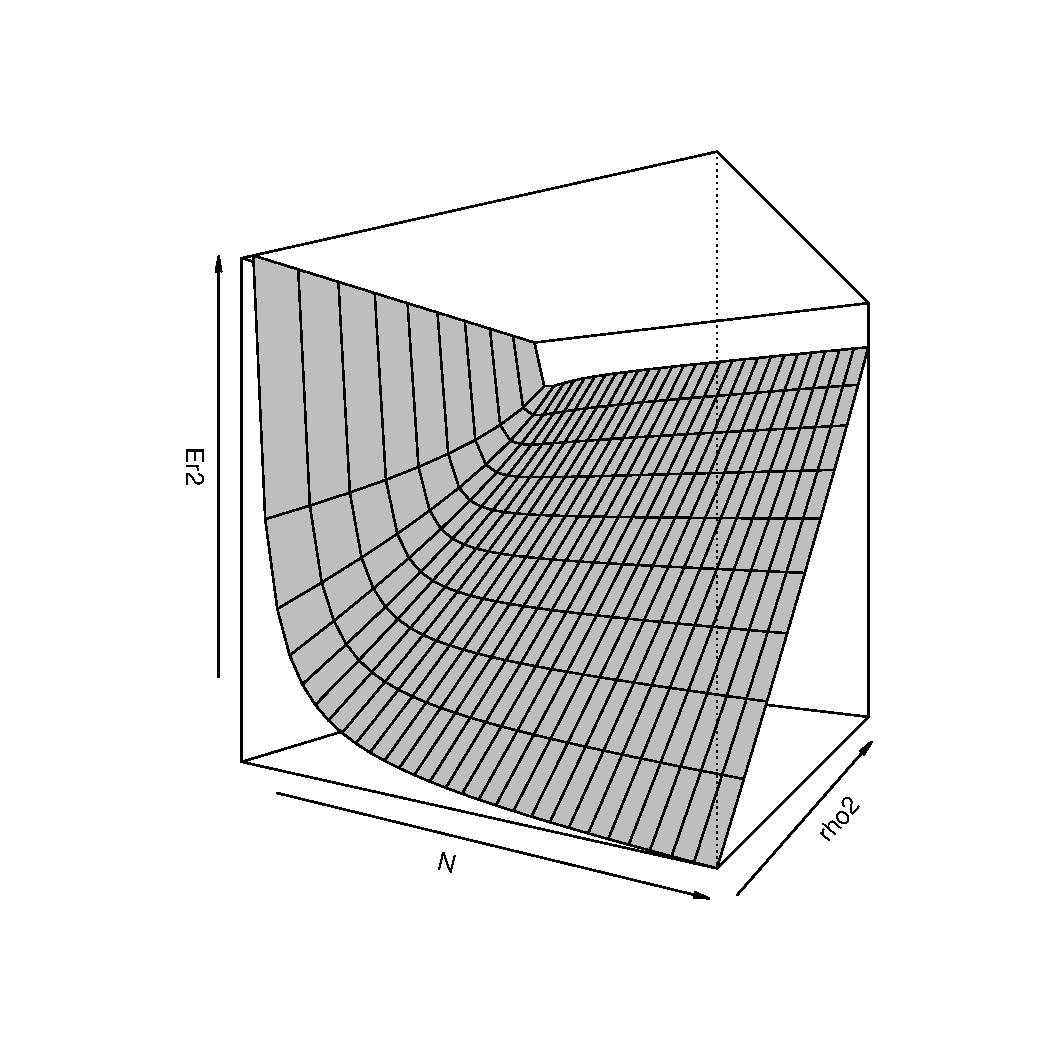
\includegraphics{2016_w10_files/figure-latex/unnamed-chunk-3-1.pdf}

\subsection{\texorpdfstring{Paketet
\texttt{cvq2}}{Paketet cvq2}}\label{paketet-cvq2}

Se: \url{http://www.r-pkg.org/pkg/cvq2}

Tror dock inte att detta äre relevant i sammanhanget. Behandlar PRESS
etc.

\subsection{Läsning av (Zou 2007)}\label{lasning-av-zou2007}

Erbjöd även SAS-kod i supplemental materials:
\url{http://dx.doi.org/10.1037/1082-989x.12.4.399.supp}

Nämner här att det fnins åtm 14 olika sätt att betrakta \(\rho^2\) (jmfr
(Rodgers and Nicewander 1988) som också refereras ihop med ytterligare
sätt).

Om man vill skapa KI för enskild \(\rho2\) funkar det ganska bra med
Fishers z (transformerar fram och tillbaka). Detta funkar dock inte vid
jämförelser mellan två olika \(\rho2\) då bakåttransformation saknas.

För \(\rho^2\) är det ännu mer komplicerat då fördelningen är så knepig.
Skriver att sådana tabulerade värden har publicerats men att de sällan
använts. Approximationer finns också som sägs funka ganska bra men som
trots allt inte kan användas för jämförelser. Approximationer som
ignorerar fördelningens skevhet har också presenterats med sedan
förkastats (James Algina 1999).

Poängterar att man inte får blanda ihop fördelning för \(r\) och
\(\sqrt{R^2}\) då den senare ju bara kan anta positiva värtden.

Finns SAS-metod: ``SAS PROC CANCORR'' och i appendix beskrivs även
implementat5ion för SPSS. Dessa bygger på approximation mha
F-fördelning.

\begin{itemize}
\tightlist
\item
  För \(\rho\):
\item
  Överlapping: Metoder som bygger på normalantagande funkar inte för
  stickprov mindre än 100. För storlek 100 - 200 täcker man \(\rho^2\)
  i\\
  \(1-\alpha\) procent av fallen men assymetrin ger skevt resultat upp
  till stickprovsstorlekar på ca 200. Med F-fördelning funkar det dock
  bra för storlekar ner till ca 15.
\item
  Ej överlappande:
\item
  För \(\rho^2\):
\item
  Funkar inte alls med normalfördelningsantagande
\item
  Funkar hyffsat med F-fördelning men testas bara för
  stickprovsstorlekar \textgreater{}= 50. Dock med \(p = 3, 6\) (men
  resultaten likvärdiga så redovisar endast för \(p = 6\) i tab 3).
\end{itemize}

Gör flera referenser till Lee 1971 för approximativ fördelning till
\(R^2\) så gissar att det kan vara värt att kolla upp. Slutsats för
\(R^2\) är att resultatet trots allt blir ungefär samma som enl (J.
Algina and Moulder 2001) (som tillämpade en mer approximativ metod).

\textbf{OBS!} Finns ett bra appendix som också förklarar den
approximativa icke-centrala F-fördelningen enl Lee 1971. Observera att
den fördelningen gäller rtansformationen ovan, där (Helland 1987) anger
Gurland 1968 som källa men med skillnaden att vi här har en
icke-centralfördelning (gissar att denna på ngt sätt är bättre då den
dessutmo är senare).

\subsection{\texorpdfstring{Paketet
\texttt{cocor}}{Paketet cocor}}\label{paketet-cocor}

Se: \url{http://www.r-pkg.org/pkg/cocor}

Paketet har också GUI dels online, dels för desktop.

\subsubsection{Läsning av (Diedenhofen and Musch
2015).}\label{lasning-av-diedenhofen2015.}

KI skapas baserat på (Zou 2007) men behandlar tyvärr bara korrelation
och inte \(\rho^2\). Går därför inte vidare med detta men kanske ändå
värt att nämna att det finns ett lättanvänt verktyg för vanlig
korrelation (gher dessutom väldigt många olika testresultat \ldots{}
kanske för många med tanke på att alla kanske inte är optimala
\ldots{}).

\subsection{Läsning av (Lee 1971)}\label{lasning-av-lee1971}

Undersöker sample distribution multiple correlation coefficient. Från
normal sample. När antalet oberoende variater udda är denna fördelning
förbunden med fördelningen för simlpe correlation. Utnyttjar att
underliggande fördelning är ickecentral beta men approximerar med
central och ickecentral F samt normalfördelning.

Poängterar att (Hotelling 1953) föreslog beräkning av
fördelningsfunktion mha rekursion (``recurrence formula'') men tyvärr
bara för udda p.

Ger (23) som en approximativ fördelningsfunktion mha ickecentral beta.
Lång formel så skriver inte ner den just nu men implementerar som
R-funktion för skoj skull:

\begin{Shaded}
\begin{Highlighting}[]
\CommentTok{# Approxinmativ F via ickecentral beta}
\NormalTok{pr2 <-}\StringTok{ }\NormalTok{function(q, n, p, rho) \{}
  
  \NormalTok{rh <-}\StringTok{ }\NormalTok{rho ^}\StringTok{ }\DecValTok{2} \NormalTok{/}\StringTok{ }\NormalTok{(}\DecValTok{1} \NormalTok{-}\StringTok{ }\NormalTok{rho ^}\StringTok{ }\DecValTok{2}\NormalTok{)}
  \NormalTok{a <-}\StringTok{ }\NormalTok{n *}\StringTok{ }\NormalTok{rh}
  \NormalTok{B <-}\StringTok{ }\NormalTok{function(shape1, shape2) stats::}\KeywordTok{pbeta}\NormalTok{(q, shape1, shape2,  }\DataTypeTok{ncp =} \NormalTok{a)}
  
  \KeywordTok{B}\NormalTok{(p, n -}\StringTok{ }\NormalTok{p) +}\StringTok{ }
\StringTok{  }\NormalTok{(a ^}\StringTok{ }\DecValTok{2} \NormalTok{/}\StringTok{ }\NormalTok{(}\DecValTok{4} \NormalTok{*}\StringTok{ }\NormalTok{n))      *}\StringTok{ }\NormalTok{(}\KeywordTok{B}\NormalTok{(p, n -}\StringTok{ }\NormalTok{p) -}\StringTok{ }\DecValTok{2} \NormalTok{*}\StringTok{ }\KeywordTok{B}\NormalTok{(p +}\StringTok{ }\DecValTok{2}\NormalTok{, n -}\StringTok{ }\NormalTok{p) +}\StringTok{ }\KeywordTok{B}\NormalTok{(p +}\StringTok{ }\DecValTok{4}\NormalTok{, n -}\StringTok{ }\NormalTok{p)) +}\StringTok{ }
\StringTok{  }\NormalTok{(a ^}\StringTok{ }\DecValTok{3} \NormalTok{/}\StringTok{ }\NormalTok{(}\DecValTok{96} \NormalTok{*}\StringTok{ }\NormalTok{n ^}\StringTok{ }\DecValTok{2}\NormalTok{)) *}\StringTok{ }\NormalTok{(}
    \NormalTok{(}\DecValTok{3} \NormalTok{*}\StringTok{ }\NormalTok{a -}\StringTok{ }\DecValTok{16}\NormalTok{) *}\StringTok{ }\KeywordTok{B}\NormalTok{(p, n -}\StringTok{ }\NormalTok{p) -}\StringTok{ }\DecValTok{12} \NormalTok{*}\StringTok{ }\NormalTok{(a -}\StringTok{ }\DecValTok{4}\NormalTok{) *}\StringTok{ }\KeywordTok{B}\NormalTok{(p +}\StringTok{ }\DecValTok{2}\NormalTok{, n -}\StringTok{ }\NormalTok{p) +}
\StringTok{    }\DecValTok{6} \NormalTok{*}\StringTok{ }\NormalTok{(}\DecValTok{3} \NormalTok{*}\StringTok{ }\NormalTok{a -}\StringTok{ }\DecValTok{8}\NormalTok{) *}\StringTok{ }\KeywordTok{B}\NormalTok{(p +}\StringTok{ }\DecValTok{4}\NormalTok{, n -}\StringTok{ }\NormalTok{p) -}\StringTok{ }\DecValTok{4} \NormalTok{*}\StringTok{ }\NormalTok{(}\DecValTok{3} \NormalTok{*}\StringTok{ }\NormalTok{a -}\StringTok{ }\DecValTok{4}\NormalTok{) *}\StringTok{ }\KeywordTok{B}\NormalTok{(p +}\StringTok{ }\DecValTok{6}\NormalTok{, n -}\StringTok{ }\NormalTok{p) +}
\StringTok{    }\DecValTok{3} \NormalTok{*}\StringTok{ }\NormalTok{a *}\StringTok{ }\KeywordTok{B}\NormalTok{(p +}\StringTok{ }\DecValTok{8}\NormalTok{, n -}\StringTok{ }\NormalTok{p)}
  \NormalTok{) }\CommentTok{# + O(n ^-3)}
\NormalTok{\}}

\NormalTok{q <-}\StringTok{ }\KeywordTok{seq}\NormalTok{(}\DecValTok{0}\NormalTok{, }\DecValTok{1}\NormalTok{, .}\DecValTok{01}\NormalTok{)}
\KeywordTok{par}\NormalTok{(}\DataTypeTok{mfrow =} \KeywordTok{c}\NormalTok{(}\DecValTok{1}\NormalTok{, }\DecValTok{2}\NormalTok{))}
\KeywordTok{plot}\NormalTok{(q, }\KeywordTok{pr2}\NormalTok{(q, }\DecValTok{10}\NormalTok{, }\DecValTok{5}\NormalTok{, }\DecValTok{0}\NormalTok{), }\DataTypeTok{type =} \StringTok{"l"}\NormalTok{, }\DataTypeTok{main =} \StringTok{"rho = 0 Större stickprov ger linje till vänster"}\NormalTok{) }
\KeywordTok{lines}\NormalTok{(q, }\KeywordTok{pr2}\NormalTok{(q, }\DecValTok{30}\NormalTok{, }\DecValTok{5}\NormalTok{, }\DecValTok{0}\NormalTok{), }\DataTypeTok{type =} \StringTok{"l"}\NormalTok{) }
\KeywordTok{lines}\NormalTok{(q, }\KeywordTok{pr2}\NormalTok{(q, }\DecValTok{50}\NormalTok{, }\DecValTok{5}\NormalTok{, }\DecValTok{0}\NormalTok{), }\DataTypeTok{type =} \StringTok{"l"}\NormalTok{) }
\KeywordTok{lines}\NormalTok{(q, }\KeywordTok{pr2}\NormalTok{(q, }\DecValTok{100}\NormalTok{, }\DecValTok{5}\NormalTok{, }\DecValTok{0}\NormalTok{), }\DataTypeTok{type =} \StringTok{"l"}\NormalTok{) }

\KeywordTok{plot}\NormalTok{(q, }\KeywordTok{pr2}\NormalTok{(q, }\DecValTok{10}\NormalTok{, }\DecValTok{5}\NormalTok{, .}\DecValTok{5}\NormalTok{), }\DataTypeTok{type =} \StringTok{"l"}\NormalTok{, }\DataTypeTok{main =} \StringTok{"rho = .5 Större stickprov ger linje till vänster"}\NormalTok{) }
\KeywordTok{lines}\NormalTok{(q, }\KeywordTok{pr2}\NormalTok{(q, }\DecValTok{30}\NormalTok{, }\DecValTok{5}\NormalTok{, .}\DecValTok{5}\NormalTok{), }\DataTypeTok{type =} \StringTok{"l"}\NormalTok{) }
\KeywordTok{lines}\NormalTok{(q, }\KeywordTok{pr2}\NormalTok{(q, }\DecValTok{50}\NormalTok{, }\DecValTok{5}\NormalTok{, .}\DecValTok{5}\NormalTok{), }\DataTypeTok{type =} \StringTok{"l"}\NormalTok{) }
\KeywordTok{lines}\NormalTok{(q, }\KeywordTok{pr2}\NormalTok{(q, }\DecValTok{100}\NormalTok{, }\DecValTok{5}\NormalTok{, .}\DecValTok{5}\NormalTok{), }\DataTypeTok{type =} \StringTok{"l"}\NormalTok{) }
\end{Highlighting}
\end{Shaded}

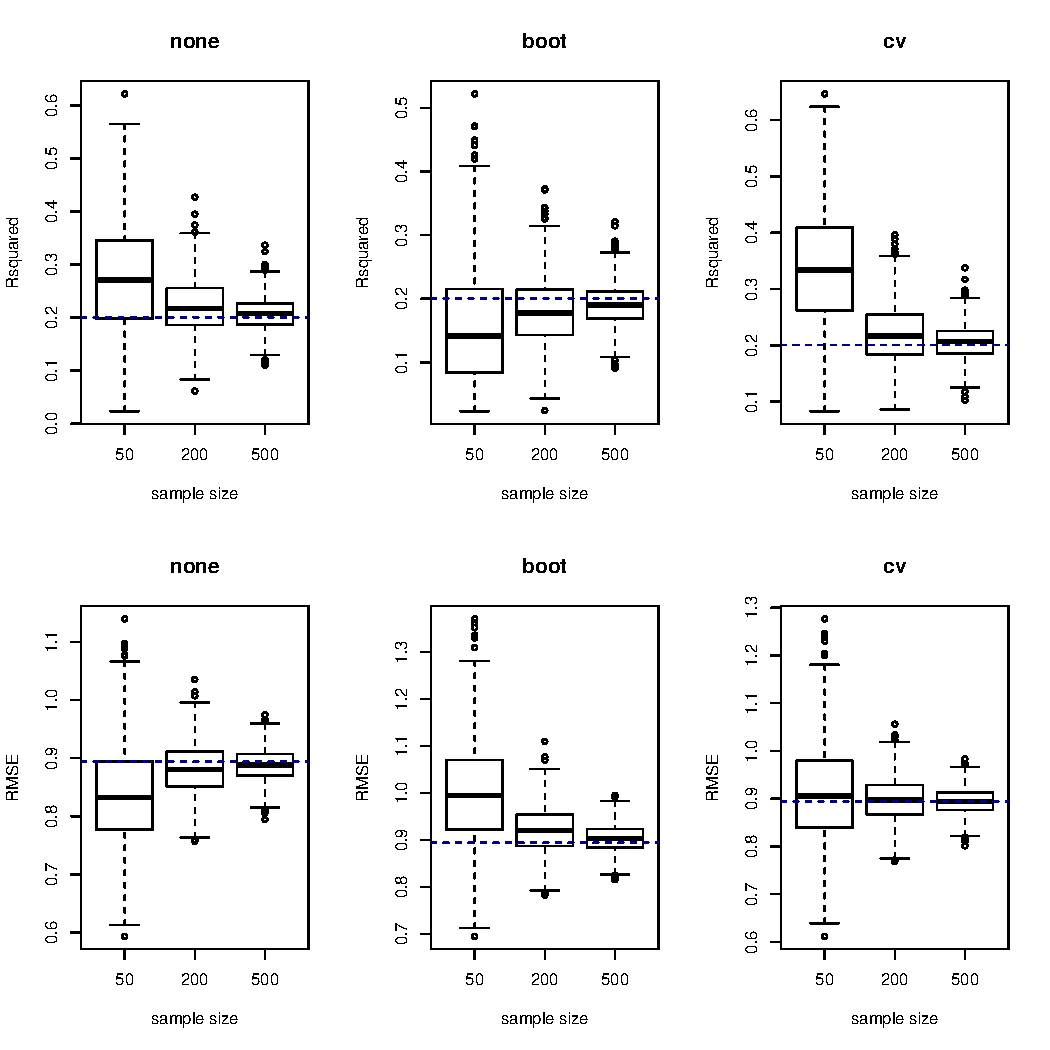
\includegraphics{2016_w10_files/figure-latex/unnamed-chunk-4-1.pdf}

Här ser vi att större stickprov ger brantare linje, vilket är korrekt.
Vi vill ju (för första bilden) att \(P(R^2 \leq 0|\rho^2 = 0) = 0\).

Vi kanske kan utöka denna jämförelse för olika p och fler rho etc?

Artiklen ger även approximationer för \(\tilde{R}^2 \sim F\) och
icke-central F men jag nöjer mig just nu med den första då den ändå inte
rör \(R^2\) direkt utan en transformation därav.

Görs även en approximation mha normalfördelning baserat på power-series
men. Görs även jmfr med Fishers z men fniner att det är en dålig metod
med för mkt bias etc. I editors note görs försök att rädda Fishers z,
går delvis men inte helt och metoder fortf sämre än F-approximationerna.

\section*{Referenser}\label{referenser}
\addcontentsline{toc}{section}{Referenser}

\hypertarget{refs}{}
\hypertarget{ref-Algina2001}{}
Algina, J., and B. C. Moulder. 2001. ``Sample Sizes for Confidence
Intervals on the Increase in the Squared Multiple Correlation
Coefficient.'' \emph{Educational and Psychological Measurement} 61 (4):
633--49.
doi:\href{https://doi.org/10.1177/00131640121971400}{10.1177/00131640121971400}.

\hypertarget{ref-Algina1999}{}
Algina, James. 1999. ``A Comparison of Methods for Constructing
Confidence Intervals for the Squared Multiple Correlation Coefficient.''
\emph{Multivariate Behavioral Research} 34 (4): 493--504.
doi:\href{https://doi.org/10.1207/S15327906MBR3404\%7B/_\%7D5}{10.1207/S15327906MBR3404\{\textbackslash{}\_\}5}.

\hypertarget{ref-Cattin1980}{}
Cattin, Philippe. 1980. ``Estimation of the Predictive Power of a
Regression Model.'' \emph{Journal of Applied Psychology} 65 (4):
407--14.
doi:\href{https://doi.org/10.1037//0021-9010.65.4.407}{10.1037//0021-9010.65.4.407}.

\hypertarget{ref-Crocker1972}{}
Crocker, Douglas C. 1972. ``Some Interpretations of the Multiple
Correlation Coefficient.'' \emph{The American Statistician} 26 (2).
Taylor \& Francis: 31--33.
doi:\href{https://doi.org/10.1080/00031305.1972.10477345}{10.1080/00031305.1972.10477345}.

\hypertarget{ref-Diedenhofen2015}{}
Diedenhofen, Birk, and Jochen Musch. 2015. ``Cocor: A Comprehensive
Solution for the Statistical Comparison of Correlations.'' \emph{PloS
One} 10 (3). Public Library of Science: e0121945.
doi:\href{https://doi.org/10.1371/journal.pone.0121945}{10.1371/journal.pone.0121945}.

\hypertarget{ref-Ezekei1929}{}
Ezekei, Mordecai. 1929. ``The Application of the Theory of Error to
Multiple and Curvilinear Correlation.'' \emph{Journal of the American
Statistical Association} 24 (165): 99--104.

\hypertarget{ref-Fisher1928}{}
Fisher, R A. 1928. ``The General Sampling Distribution of the Multiple
Correlation Coefficient.'' \emph{Proceedings of the Royal Society of
London A: Mathematical, Physical and Engineering Sciences} 121 (788):
654--73.
\url{http://rspa.royalsocietypublishing.org/content/121/788/654.abstract}.

\hypertarget{ref-Fisher1924}{}
Fisher, R a. 1924. ``The distribution of the partial correlation
coefficient.'' \emph{Metron} 3 (3-4): 329--32.

\hypertarget{ref-Helland1987}{}
Helland, Inge S. 1987. ``On the Interpretation and Use of R2 in
Regression Analysis.'' \emph{Biometrics} 43 (1). {[}Wiley, International
Biometric Society{]}: 61--69.
doi:\href{https://doi.org/10.2307/2531949}{10.2307/2531949}.

\hypertarget{ref-Hotelling1953}{}
Hotelling, Harold. 1953. ``New Light on the Correlation Coefficient and
its Transforms Author(s): Harold Hotelling.'' \emph{Journal of the Royal
Statistical Society. Series B (Methodological),} 15 (2): 296--193--232.

\hypertarget{ref-Kramer1963}{}
Kramer, K H. 1963. ``Tables for Constructing Confidence Limits on the
Multiple Correlation Coefficient.'' \emph{Journal of the American
Statistical Association} 58 (304). {[}American Statistical Association,
Taylor \& Francis, Ltd.{]}: 1082--5.
doi:\href{https://doi.org/10.2307/2283334}{10.2307/2283334}.

\hypertarget{ref-Kreke2015}{}
Kreke, Joseph G, Sangeet Khemlani, and Greg Trafton. 2015. ``pAnalysis:
Benchmarking and Rescaling R2 using Noise Percentile Analysis.''
\url{https://cran.r-project.org/package=pAnalysis}.

\hypertarget{ref-Lee1971}{}
Lee, Yoong-Sin. 1971. ``Some Results on the Sampling Distribution of the
Multiple Correlation Coefficient.'' \emph{Journal of the Royal
Statistical Society. Series B (Methodological)} 33 (1). {[}Royal
Statistical Society, Wiley{]}: 117--30.
\url{http://www.jstor.org/stable/2986012}.

\hypertarget{ref-Montgomery1973}{}
Montgomery, David B, and Donald G Morrison. 1973. ``A Note on Adjusting
R2.'' \emph{The Journal of Finance} 28 (4): 1009--13.

\hypertarget{ref-Nakagawa1992}{}
Nakagawa, Shigekazu, and Naoto Niki. 1992. ``Distribution of the sample
correlation coefficient for nonnormal populations.'' \emph{Journal of
the Japanese Society of Computational Statistics} 5 (1): 1--19.
doi:\href{https://doi.org/10.5183/jjscs1988.5.1}{10.5183/jjscs1988.5.1}.

\hypertarget{ref-Olkin1958}{}
Olkin, Ingram, and J.W. Pratt. 1958. ``Unbiased estimation of certain
correlation coefficients.'' \emph{The Annals of Mathematical Statistics}
29 (1): 201--11.
doi:\href{https://doi.org/10.2307/2237306}{10.2307/2237306}.

\hypertarget{ref-Ozer1985}{}
Ozer, Daniel J. 1985. ``Correlation and the coefficient of
determination.'' \emph{Psychological Bulletin} 97 (2): 307--15.
doi:\href{https://doi.org/10.1037/0033-2909.97.2.307}{10.1037/0033-2909.97.2.307}.

\hypertarget{ref-Raju1999}{}
Raju, N S, R Bilgic, J E Edwards, and P F Fleer. 1999. ``Accuracy of
Population Validity and Cross-Validity Estimation: An Empirical
Comparison of Formula-Based, Traditional Empirical, and Equal Weights
Procedures.'' \emph{Applied Psychological Measurement} 23 (2): 99--115.
doi:\href{https://doi.org/10.1177/01466219922031220}{10.1177/01466219922031220}.

\hypertarget{ref-Raju1997}{}
Raju, Nambury S, Reyhan Bilgic, Jack E Edwards, and Paul F Fleer. 1997.
``Methodology Review: Estimation of population validity and
cross-validity, and the use of equal weights in prediction.''
\emph{Applied Psychological Measurement} 21 (4): 291--305.

\hypertarget{ref-Rodgers1988}{}
Rodgers, Joseph Lee, and W. Alan Nicewander. 1988. ``Thirteen Ways to
Look at the Correlation Coefficient.'' \emph{The American Statistician}
42 (1): 59--66.
doi:\href{https://doi.org/10.2307/2685263}{10.2307/2685263}.

\hypertarget{ref-Skidmore2011}{}
Skidmore, Susan Troncoso, and Bruce Thompson. 2011. ``Choosing the Best
Correction Formula for the Pearson r 2 Effect Size.'' \emph{The Journal
of Experimental Education} 79 (3): 257--78.
doi:\href{https://doi.org/10.1080/00220973.2010.484437}{10.1080/00220973.2010.484437}.

\hypertarget{ref-Steiger1992}{}
Steiger, James H., and Rachel T. Fouladi. 1992. ``R2: A computer program
for interval estimation, power Calculations, sample size estimation, and
hypothesis testing in multiple regression.'' \emph{Behavior Research
Methods, Instruments, \& Computers} 24 (4): 581--82.
doi:\href{https://doi.org/10.3758/BF03203611}{10.3758/BF03203611}.

\hypertarget{ref-Walck2007}{}
Walck, Christian. 2007. ``Hand-book on STATISTICAL DISTRIBUTIONS for
experimentalists.''
\href{http://www.stat.rice.edu/\%7B~\%7Ddobelman/textfiles/DistributionsHandbook.pdf}{http://www.stat.rice.edu/\{\textasciitilde{}\}dobelman/textfiles/DistributionsHandbook.pdf}.

\hypertarget{ref-Wasserstein2016}{}
Wasserstein, Ronald L., and Nicole A. Lazar. 2016. ``The ASA's statement
on p-values: context, process, and purpose.'' \emph{The American
Statistician}, March. Taylor \& Francis, 00--00.
doi:\href{https://doi.org/10.1080/00031305.2016.1154108}{10.1080/00031305.2016.1154108}.

\hypertarget{ref-Wherry1931}{}
Wherry, R. 1931. ``A new formula for predicting the shrinkage of the
coefficient of multiple correlation.'' \emph{The Annals of Mathematical
Statistics} 2 (4): 440--57.
\url{http://www.jstor.org/stable/2957681$/backslash$npapers2://publication/uuid/F3D4916B-BB98-4094-A459-DF4387AC9610}.

\hypertarget{ref-Wishart1931}{}
Wishart, Author J, T Kondo, and E M Elderton. 1931. ``The Mean and
Second Moment Coefficient of the Multiple Correlation Coefficient, in
Samples from a Normal Population.'' \emph{Biometrika} 22 (3/4): 353--76.

\hypertarget{ref-Zou2007}{}
Zou, Guang Yong. 2007. ``Toward using confidence intervals to compare
correlations.'' \emph{Psychological Methods} 12 (4). Department of
Epidemiology; Biostatistics, Schulich School of Medicine; Dentistry,
University of Western Ontario, London, ON, Canada gzou@robarts.ca; Zou,
Guang Yong,London,Canada,N6A 5C1,Department of Epidemiology;
Biostatistics, Schulich School: American Psychological Association:
399--413.
doi:\href{https://doi.org/http://dx.doi.org/10.1037/1082-989X.12.4.399}{http://dx.doi.org/10.1037/1082-989X.12.4.399}.

\end{document}
